\documentclass[12pt]{article}
\usepackage{graphicx}
\usepackage{xcolor}
\usepackage{hyperref}
\usepackage{wasysym}
\usepackage{mathrsfs}
\usepackage[calc]{datetime2}
\usepackage{boondox-cal}
\usepackage{bm} % For bold math symbols
\usepackage{amsmath}
\usepackage{amssymb}
\usepackage{cancel}
\usepackage{tikz}
\usepackage{subcaption}
\usepackage[margin=0.75in]{geometry}

\usetikzlibrary{arrows}

\DTMsavenow{now}
\DTMsavedate{DueDate}{2024-02-6}

\newcount\daystilldue
\newcount\hourstilldue
\newcount\minutestilldue

% Calculate the difference in days
\DTMsaveddatediff{DueDate}{now}{\daystilldue}

% Calculate the difference in hours and minutes
\hourstilldue=\DTMfetchhour{DueDate}
\advance\hourstilldue by -\DTMfetchhour{now}
\minutestilldue=\DTMfetchminute{DueDate}
\advance\minutestilldue by -\DTMfetchminute{now}

% Adjust for negative values
\ifnum\hourstilldue<0
  \advance\hourstilldue by 24
  \advance\daystilldue by -1
\fi
\ifnum\minutestilldue<0
  \advance\minutestilldue by 60
  \advance\hourstilldue by -1
\fi

\newcommand{\TimeUntilDue}{
  \ifnum\daystilldue<4
    \textcolor{red}{
    \number\daystilldue\ days - 
    \number\hourstilldue\ hours - 
    \number\minutestilldue\ min until deadline!!
  }
\else
    \number\daystilldue\ days - 
    \number\hourstilldue\ hours - 
    \number\minutestilldue\ min until deadline
  \fi
}

\newcommand{\delCross}[1]{
  \left[\hat a_x\left(\frac{\partial\bm{#1}_z}{\partial y} - \frac{\partial\bm{#1}_y}{\partial z}\right) - \hat a_y\left( \frac{\partial\bm{#1}_z}{\partial x} - \frac{\partial\bm{#1}_x}{\partial z}  \right) + \hat a_z\left( \frac{\partial\bm{#1}_y}{\partial x} -  \frac{\partial\bm{#1}_x}{\partial y}\right)\right]
}
\begin{document}

\newcommand{\Cross}[2]{
\hat a_x(#1_2#2_3 -#1_3#2_2) -\hat a_y(#1_1#2_3-#1_3#2_1) + \hat a_z(#1_1#2_2-#1_2#2_1) 
}
\title{ECE 6310 - Advanced Electromagnetic Fields: Homework Set \#2}
\author{Miguel Gomez}
%\date{\TimeUntilDue}
\maketitle

%\begin{center}
%  $\mathcal{ABCDEFGHIJKLMNOPQRSTUVWXYZ}$\\
%$\mathscr{ABCDEFGHIJKLMNOPQRSTUVWXYZ}$
%\end{center}
\section{Preliminaries}

In this document, we use standard notation for electromagnetic theory. Key equations and concepts are summarized below:

\subsection*{Vector Notation}
\begin{itemize}
  \item $\bm{\mathcal{E}}$: Electric field intensity
  \item $\bm{\mathcal{H}}$: Magnetic field intensity
  \item $\bm{\mathcal{D}}$: Electric flux density
  \item $\bm{\mathcal{B}}$: Magnetic flux density
  \item $\bm{\mathcal{J}}$: Current density
  \item $\rho_v$: Volume charge density
\end{itemize}

\subsection*{Differential Operators}
\begin{itemize}
  \item $\nabla \cdot\ \ $: Divergence of a vector field
  \item $\nabla \times\ \ $: Curl of a vector field
  \item $\nabla\ \ $: Gradient of a scalar field
  \item $\partial_i\ \ $: Partial derivative with respect to the independent basis element $i$
\end{itemize}

\subsection*{Maxwell's Equations}
In integral form, Maxwell's equations are given by:
\begin{align}
  \oint_{\partial V} \bm{\mathcal{E}} \cdot d\bm{\mathcal{l}} &= - \frac{d}{dt} \int_{V} \bm{\mathcal{B}} \cdot d\bm{\mathcal{S}} & \text{(Faraday's Law of Induction)} \\
  \oint_{\partial V} \bm{\mathcal{H}} \cdot d\bm{\mathcal{l}} &= \int_{V} \bm{\mathcal{J}} \cdot d\bm{\mathcal{S}} + \frac{d}{dt} \int_{V} \bm{\mathcal{D}} \cdot d\bm{\mathcal{S}} & \text{(Ampère's Circuital Law)} \\
  \oiint_{\partial V} \bm{\mathcal{D}} \cdot d\bm{\mathcal{S}} &= \int_{V} \rho_v dV & \text{(Gauss's Law for Electricity)} \\
  \oiint_{\partial V} \bm{\mathcal{B}} \cdot d\bm{\mathcal{S}} &= 0 & \text{(Gauss's Law for Magnetism)}
\end{align}

\subsection*{Other Relevant Equations}
\begin{itemize}
  \item Continuity Equation: $\nabla \cdot \bm{\mathcal{J}} + \partial_t \rho_v = 0$
  \item Relationship between $\bm{\mathcal{E}}$, $\bm{\mathcal{D}}$: $\bm{\mathcal{D}} = \epsilon \bm{\mathcal{E}}$
  \item Relationship between $\bm{\mathcal{H}}$, $\bm{\mathcal{B}}$: $\bm{\mathcal{B}} = \mu \bm{\mathcal{H}}$
\end{itemize}

\subsection*{Boundary Conditions}
Discuss the boundary conditions for $\bm{\mathcal{E}}$, $\bm{\mathcal{H}}$, $\bm{\mathcal{D}}$, and $\bm{\mathcal{B}}$ at interfaces between different media.
\newpage
\section*{Problem 3.2}
Verify that (3-28a) and (3-28b) are solutions to (3-26a)\\
To solve this problem, we can first set up the expressions we need
\begin{itemize}
\item[(3-26a)]
  \begin{equation}
    \frac{d^2f}{dx^2} = -\beta_x^2f\label{deriv_expression}
  \end{equation}
\item[(3-28a)]
  \begin{align*}
    f(x) &= A_1e^{-j\beta_xx} + B_1e^{j\beta_xx}\\
    \frac{d}{dx}f(x) &= -j\beta_xA_1e^{-j\beta_xx} + j\beta_xB_1e^{j\beta_xx}\\
    \frac{d^2}{dx^2}f(x) &= (-j\beta_x)^2A_1e^{-j\beta_xx} + (j\beta_x)^2B_1e^{j\beta_xx}\\
    \frac{d^2}{dx^2}f(x) &= -\beta_x^2A_1e^{-j\beta_xx} - \beta_x^2B_1e^{j\beta_xx}\\
         &= - \beta_x^2(A_1e^{-j\beta_xx} + B_1e^{j\beta_xx})\\
         &=- \beta_x^2 f(x)
  \end{align*}
  \item[(3-28b)]
\begin{align*}
  f(x) &= C_1\cos{(\beta_xx)} + D_1\sin{(\beta_xx)}\\
  \frac{d}{dx}f(x) &= -\beta_xC_1\sin{(\beta_xx)} + \beta_xD_1\cos{(\beta_xx)} \\
  \frac{d^2}{dx^2}f(x) &= -\beta_x^2C_1\cos{(\beta_xx)} - \beta_x^2D_1\sin{(\beta_xx) } \\
       &= - \beta_x^2(C_1\cos{(\beta_xx)} + D_1\sin{(\beta_xx) }) \\
       &= - \beta_x^2 f(x)
\end{align*}
\end{itemize}
\section*{Problem 4.2}
Using Maxwell’s equations, find the magnetic field components for the wave whose electric field is given in Example 4-1. Compare your answer with that obtained in the solution of Example 4-1.\\
The expression for the magnetic field in terms of the electric field is:
\begin{align*}
  H &= -\frac{1}{j\omega\mu}\delCross{E}
\end{align*}
Example 4-1 shows the electric field as:
\begin{align*}
  E = \hat a_y(E_0^+e^{-j\beta z} + E_0^-e^{+j\beta z}) = \hat a_y(E_y^+ + E_y^-)
\end{align*}
Since it only has a $y$ component, we can take all the parts that do not have a $y$ component and set them to 0.
\begin{align*}
 H &= -\frac{1}{j\omega\mu} \left[\hat a_x\left(\textcolor{red}{\cancelto{\textcolor{black}{0}}{\textcolor{black}{\frac{\partial\bm{E}_z}{\partial y}}}} - \frac{\partial\bm{E}_y}{\partial z}\right) - \hat a_y\left( \textcolor{red}{\cancelto{\textcolor{black}{0}}{\textcolor{black}{\frac{\partial\bm{E}_z}{\partial x}}}} - \textcolor{red}{\cancelto{\textcolor{black}{0}}{\textcolor{black}{\frac{\partial\bm{E}_x}{\partial z}}}}  \right) + \hat a_z\left( \frac{\partial\bm{E}_y}{\partial x} -  \textcolor{red}{\cancelto{\textcolor{black}{0}}{\textcolor{black}{\frac{\partial\bm{E}_x}{\partial y}}}}\right)\right]\\
  &= -\frac{1}{j\omega\mu}  \left[-\hat a_x\frac{\partial\bm{E}_y}{\partial z} + \hat a_z\frac{\partial\bm{E}_y}{\partial x}\right]
\end{align*}
We can also get rid of the partial w.r.t. $x$ since $E$ does not have a dependence on $x$.
\begin{align*}
  H &= -\frac{1}{j\omega\mu}  \left[-\hat a_x\frac{\partial\bm{E}_y}{\partial z} + \hat a_z\textcolor{red}{\cancelto{\textcolor{black}{0}}{\textcolor{black}{\frac{\partial\bm{E}_y}{\partial x}}}}\ \ \ \right]\\
  H &= \frac{1}{j\omega\mu}  \left[\hat a_x\frac{\partial\bm{E}_y}{\partial z} \right]\\
  H &= \frac{1}{j\omega\mu}  \left[\hat a_x\frac{\partial}{\partial z}(E_y^+ + E_y^-) \right]\\
  H &= \frac{1}{j\omega\mu}  \left[\hat a_x(-j\beta E_0^+e^{-j\beta z} + j\beta E_0^-e^{+j\beta z}) \right]\\
  H &= \frac{\beta}{\omega\mu}  \left[\hat a_x(E_0^+e^{-j\beta z} - E_0^-e^{+j\beta z}) \right]
\end{align*}
Given the result here, we can infer that:
\begin{align*}
  \eta &= \frac{\omega \mu}{\beta} = \frac{\omega \mu}{\omega \sqrt{\mu\epsilon}} = \sqrt{\frac{\mu^2}{\mu\epsilon}}\\
  &= \sqrt{\frac{\mu}{\epsilon}}  
\end{align*}
which is the expected impedance of free space. 
\section*{Problem 4.22}
Sea water is an important medium in communication between submerged submarines or between submerged submarines and receiving and transmitting stations located above the surface of the sea. Assuming the constitutive electrical parameters of the sea are $\sigma = 4 \frac{S}{m}$, $\epsilon_r = 81$, $\mu_r = 1$, and $f = 104 Hz$, find the following:\\
Before we start, it would be good to get the following value to start:
\begin{align*}
  \left(\frac{\sigma}{\omega\epsilon}\right)^2 &= \left(\frac{4}{208\pi\cdot 10^4\cdot 81\cdot 8.854}\cdot10^{12}\right)^2\\
                                               &= \left(\frac{4}{208\pi\cdot 81\cdot 8.854}\cdot10^{8}\right)^2 \\
                                               &= 7.285e^5 \gg 1
\end{align*}
Given this result, we can take the parameters of the sea to be a good conductor. As such, $\alpha \approx \beta$.
\begin{itemize}
\item[(a)] Complex propagation constant $\gamma \frac{1}{m}$.
  \begin{align*}
    \gamma &= \alpha + j\beta = \sqrt{\frac{\omega \mu\sigma}{2}}(1+j)\\
    &=0.3974(1+j)
  \end{align*}
\item[(b)] Phase velocity $v \frac{m}{s}$.
  \begin{align*}
    v &= \frac{\omega}{\beta} = \frac{\omega}{\sqrt{\frac{\omega \mu\sigma}{2}}}\\
      &= \sqrt{\frac{2\omega^2}{\omega \mu\sigma}} = \sqrt{\frac{2\omega}{\mu\sigma}}\\
      &=1.581e^5 \left[\frac{m}{s}\right]
  \end{align*}
\item[(c)] Wavelength $\lambda\ [m]$.
  \begin{align*}
    \lambda &= \frac{2\pi}{\beta} = 2\pi\sqrt{\frac{2}{\omega\mu\sigma}}\\
            &= \sqrt{\frac{8\pi^2}{2\pi f\mu\sigma}} = \sqrt{\frac{4\pi}{f\mu\sigma}}\\
            &= 15.81 [m]
  \end{align*}
\item[(d)] Attenuation constant $\alpha \frac{N}{m}$.
  \begin{align*}
    \alpha &= \sqrt{\frac{\omega \mu\sigma}{2}}=\sqrt{\pi f \mu\sigma}\\
           & = 0.3974 \left[\frac{N}{m}\right]
  \end{align*}
\item[(e)] Skin depth $\delta\ [m]$.
  \begin{align*}
    \delta &= \frac{1}{\alpha} = \sqrt{\frac{2}{\omega \mu\sigma}}\\
    & = \frac{1}{0.3974} = 2.52\ [m]
  \end{align*}
\end{itemize}


\section*{Problem 4.26}
In a source-free, free-space region, the complex magnetic field of a time-harmonic field is represented by:
\begin{align*}
  \bm{H} &= \left[ \hat{a}_x(1+j) + \hat{a}_z\left(\sqrt{2}e^{-j \frac{\pi}{4}}\right)   \right]\frac{E_0}{\eta_0}e^{-j \beta_0y}
\end{align*}
where $E_0$ is a constant and $\eta_0$ is the intrinsic impedance of free space. Determine the:
\begin{itemize}
\item[(a)] Polarization of the wave (linear, circular, or elliptical). Justify your answer.\\
  Since the $z$ component of $H$ has a quarter $\pi$ rotation advancement, we can replace the quarter rotation using Eulers equation. A quarter turn is one of the simpler ones to replace since the real and imaginary components are both $\frac{\sqrt{2}}{2}$.
  \begin{align*}
    e^{-j \frac{\pi}{4}} &= \cos{\left(\frac{\pi}{4}\right)} + j\sin{\left(\frac{\pi}{4}\right)}\\
                         &= \frac{\sqrt{2}}{2} + j\frac{\sqrt{2}}{2} = \frac{\sqrt{2}}{2}(1+j)\\
    \bm{H} &= \left[ \hat{a}_x(1+j) + \hat{a}_z\left(\sqrt{2}\left(\frac{\sqrt{2}}{2}(1+j)\right)\right)   \right]\frac{E_0}{\eta_0}e^{-j \beta_0y}\\
    \bm{H} &= \left[ \hat{a}_x(1+j) + \hat{a}_z(1+j)   \right]\frac{E_0}{\eta_0}e^{-j \beta_0y}
  \end{align*}
  \begin{align*}
    \bm{H} &= \left[ \hat{a}_x + \hat{a}_z\right](1+j)\frac{E_0}{\eta_0}e^{-j \beta_0y}
  \end{align*}
  Since the vector contains components that are equivalent in their behavior, the polarization of the wave is linear.
\item[(b)] Sense of rotation, if any.\\
  No sense of rotation since the polarization is linear.
\item[(c)] Corresponding electric field.
  \begin{align*}
    E &= -\eta_0 \hat k \times H\\
      &= -\eta_0[\Cross{a}{H}]
  \end{align*}
  Since we have the $y$ direction as the propagation direction, we can replace the first and third components of $\hat a$ with $0$.
  \begin{align*}
    &= -\eta_0[\hat a_x(1\cdot H_3 -0\cdot H_2) -\hat a_y(0\cdot H_3-0\cdot H_1) + \hat a_z(0\cdot H_2-1\cdot H_1) ]\\
    &= -\eta_0[\hat a_xH_3  - \hat a_zH_1 ]\\
    H_1 &= H_3 \\
    \therefore E &= -\eta_0[\hat a_x  - \hat a_z](1+j)\frac{E_0}{\eta_0}e^{-j \beta_0y}\\
    &= -E_0[\hat a_x  - \hat a_z](1+j)e^{-j \beta_0y}
  \end{align*}
\end{itemize}

\section*{Problem 5.4}
A vertical interface is formed by having free space to its left and a lossless dielectric medium to its right with $\epsilon = 4\epsilon_0$ and $\mu = \mu_0$ , as shown in Figure P5-4. The incident electric field of a uniform plane wave traveling in the free-space medium and incident normally upon the interface has a value of $2\cdot 10^{−3} \frac{V}{m}$ right before it strikes the boundary. At a frequency of $3 GHz$, find the:

\begin{center}
\begin{tikzpicture}[scale=1.5, axis/.style={->, >=stealth'}]

% Draw the shaded area
\fill[gray!40] (0,-1.5) -- (1.5,-1.5) -- (1.5,1.5) -- (0,1.5) -- cycle;
% Define the axis
\draw[axis] (0,0)  -- (2,0) node(xline)[right] {$z$};
\draw[axis] (0,0) -- (0,2) node(yline)[above] {$x$};

% Draw the circle at the origin
\draw (0,0) circle (3.5pt);
\fill[black] (0,0) circle (1.75pt);

% Place the epsilon and mu labels
\node at (-0.5,1) {$\varepsilon_0, \mu_0$};
\node at (1,1) {$4\varepsilon_0, \mu_0$};

% Draw the y axis
\draw[axis] (0,0) -- (0,-1.5) node(yline)[below] {$y$};

% Label the figure
\node at (0.5,-2.5) {\textbf{Figure P5-4}};

\end{tikzpicture}

\end{center}
\begin{itemize}
\item[(a)] Reflection coefficient.\\
  \begin{align*}
    \eta &= \sqrt{\frac{\mu}{\epsilon}}\\
    \eta_1 &= \sqrt{\frac{\mu_0}{\epsilon_0}} = \eta_0\\
    \eta_2 &= \sqrt{\frac{\mu_2}{\epsilon_2}\frac{\mu_0}{4\epsilon_0}} = \frac{1}{2}\eta_0\\
    \Gamma &= \frac{\eta_2-\eta_1}{\eta_2 + \eta_1} = \frac{.5 - 1}{.5 + 1} = -\frac{1}{3}
  \end{align*}
\item[(b)] SWR in the free-space medium.\\
  \begin{align*}
    swr &= \frac{1 + |\Gamma|}{1 - |\Gamma|}\\
        &= \frac{1 + .333\mathellipsis}{1 - .333\mathellipsis} = \frac{\frac{4}{3}}{\frac{2}{3}}\\
        &= \frac{4}{2} = 2
  \end{align*}
\item[(c)] Positions (in meters) in the free-space
medium where the electric field maxima
and minima occur.\\
\begin{align*}
  |\mathbf{E}^{tot}| &= |E_0 (e^{-j \beta z} + \Gamma e^{j \beta z})| = |E_0 e^{j \beta z}||(e^{-2j \beta z} + \Gamma)|\\
  |e^{j \beta z}| &= 1\\
  &= |E_0 ||(e^{-2j \beta z} + \Gamma)|
\end{align*}
The only thing in the expression above that changes with z is the exponential, equivalent to:
\begin{align*}
  e^{-2j\beta z} &= \cos{(-2\beta z)}
\end{align*}
This is maximum when:
\begin{align*}
  -2 \beta z &= 2 \pi n\ \ \ |\ n\in\mathbb{Z}^+\\
  z &= -\frac{\pi n}{\beta}\\
  \beta &= \frac{2\pi}{\lambda} = \frac{2\pi3e9}{3e8} = 62.831\\
  z &= -\frac{\pi n}{\beta} = -\frac{\pi n}{ 62.831} = - 50\ [mm]
\end{align*}
This is minimum when:
\begin{align*}
  -2 \beta z &= \pi n\ \ \ |\ n\in\mathbb{Z}^+\\
  z &= -\frac{\pi n}{2\beta} \\
  z &= -\frac{\pi n}{2\beta} = -\frac{\pi n}{2\cdot 62.831} = - 25\ [mm]
\end{align*}
Values are in reference to the 0 point origin at the boundary, oriented towards the media. Therefore in free-space, all values would be negative in z.

\item[(d)] Max and min values of the electric field in the free-space medium.
\begin{align*}
  |\mathbf{E}^{tot}| &= |E_0 e^{j \beta z}||(e^{-2j \beta z} + \Gamma)|\\
  |\mathbf{E}^{max}| &=  |E_0 e^{j \beta (-.05)}||(e^{-2j \beta (-.05)} + \Gamma)|\\
                     &= \frac{8}{3}\ \left[\frac{mV}{m}\right]\\
  |\mathbf{E}^{min}| &=  |E_0 e^{j \beta (-.05)}||(e^{-2j \beta (-.05)} - \Gamma)|\\
                     &= \frac{4}{3}\ \left[\frac{mV}{m}\right]
\end{align*}  
\end{itemize}
\newpage
\section*{Problem 5.9}
A uniform plane wave traveling in air is incident normally on a half space occupied by a lossless dielectric medium of relative permittivity of 4. The reflections can be eliminated by placing another dielectric slab, $\frac{\lambda}{4}$ thick, between the air and the original dielectric medium, as shown in Figure P5-9. To accomplish this, the intrinsic impedance $\eta_1$ of the slab must be equal to $\sqrt{\eta_0\eta_2}$ where $\eta_0$ and $\eta_2$ are, respectively, the intrinsic impedances of air and the original dielectric medium. Assuming that the relative permeabilities of all the media are unity, what should the relative permittivity of the dielectric slab be to accomplish this?
\begin{center}
\begin{tikzpicture}[scale=1.5, axis/.style={->, >=stealth'}]

% Draw the shaded area
\fill[gray!40] (0,-1.5) -- (1.5,-1.5) -- (1.5,1.5) -- (0,1.5) -- cycle;
\fill[gray!60] (1,-1.5) -- (2,-1.5) -- (2,1.5) -- (1,1.5) -- cycle;
% Define the axis
\draw[axis] (-.5,0)  -- (2.75,0) node(xline)[right] {};
\draw[axis] (0,0) -- (0,2) node(yline)[above] {};
\draw[axis] (0,.5) -- (1,.5) node(yline)[] {};
\node at (.5,.7) {$\frac{\lambda_1}{4}$};

% Draw the circle at the origin
\draw (0,0) circle (3.5pt);
\fill[black] (0,0) circle (1.75pt);

% Place the epsilon and mu labels
\node at (-0.5,1.25) {$\eta_0$};
\node at (.5,1.25) {$\eta_1$};
\node at (.5,-.5) {$\epsilon_{r1}=?$};
\node at (1.5,1.25) {$\eta_2$};
\node at (1.5,-.5) {$\epsilon_{r2}=4$};

% Draw the y axis
\draw[axis] (0,0) -- (0,-2) node(yline)[below] {};

% Label the figure
\node at (0.5,-2.5) {\textbf{Figure P5-9}};

\end{tikzpicture}
\end{center}
This problem is a simple one. First we set the expressions for each of the impedances using the equation from \cite{balanis_2012}:
\begin{align*}
  \eta_0 &= \sqrt{\frac{\mu_0}{\epsilon_0}}\\
  \eta_1 &= \sqrt{\frac{\mu_{r1}\mu_{0}}{\epsilon_{r1}\epsilon_{0}}} = \sqrt{\frac{\mu_{r1}}{\epsilon_{r1}}}\eta_0\\
  \eta_2 &= \sqrt{\frac{\mu_{r2}\mu_{0}}{\epsilon_{r2}\epsilon_{0}}} = \sqrt{\frac{\mu_{r2}}{\epsilon_{r2}}}\eta_0
\end{align*}
Plugging in the values for what we know:
\begin{align*}
  \eta_2 &= \sqrt{\frac{1}{4}}\eta_0 = \frac{1}{2}\eta_0\\
  \eta_1 &= \sqrt{\frac{\mu_{r1}}{\epsilon_{r1}}}\eta_0 = \sqrt{\eta_0\eta_2} = \sqrt{\frac{1}{2}\eta_0^2} = \sqrt{\frac{1}{2}}\ \eta_0
\end{align*}
Now we set the expression for $\eta_1$ equal to the expression we have, and solve for the permittivity:
\newpage
\begin{align*}
  \eta_1 = \sqrt{\frac{\mu_{r1}}{\epsilon_{r1}}}\eta_0 &= \sqrt{\frac{1}{2}}\ \eta_0\\
  \therefore\ \ \sqrt{\frac{\mu_{r1}}{\epsilon_{r1}}} &= \sqrt{\frac{1}{2}}
\end{align*}
If we have $\mu_{r1} = 1$ then we can say that the relative permittivity of the middle slab should be $2$.
\begin{center}
\begin{figure}[h]
    \centering
    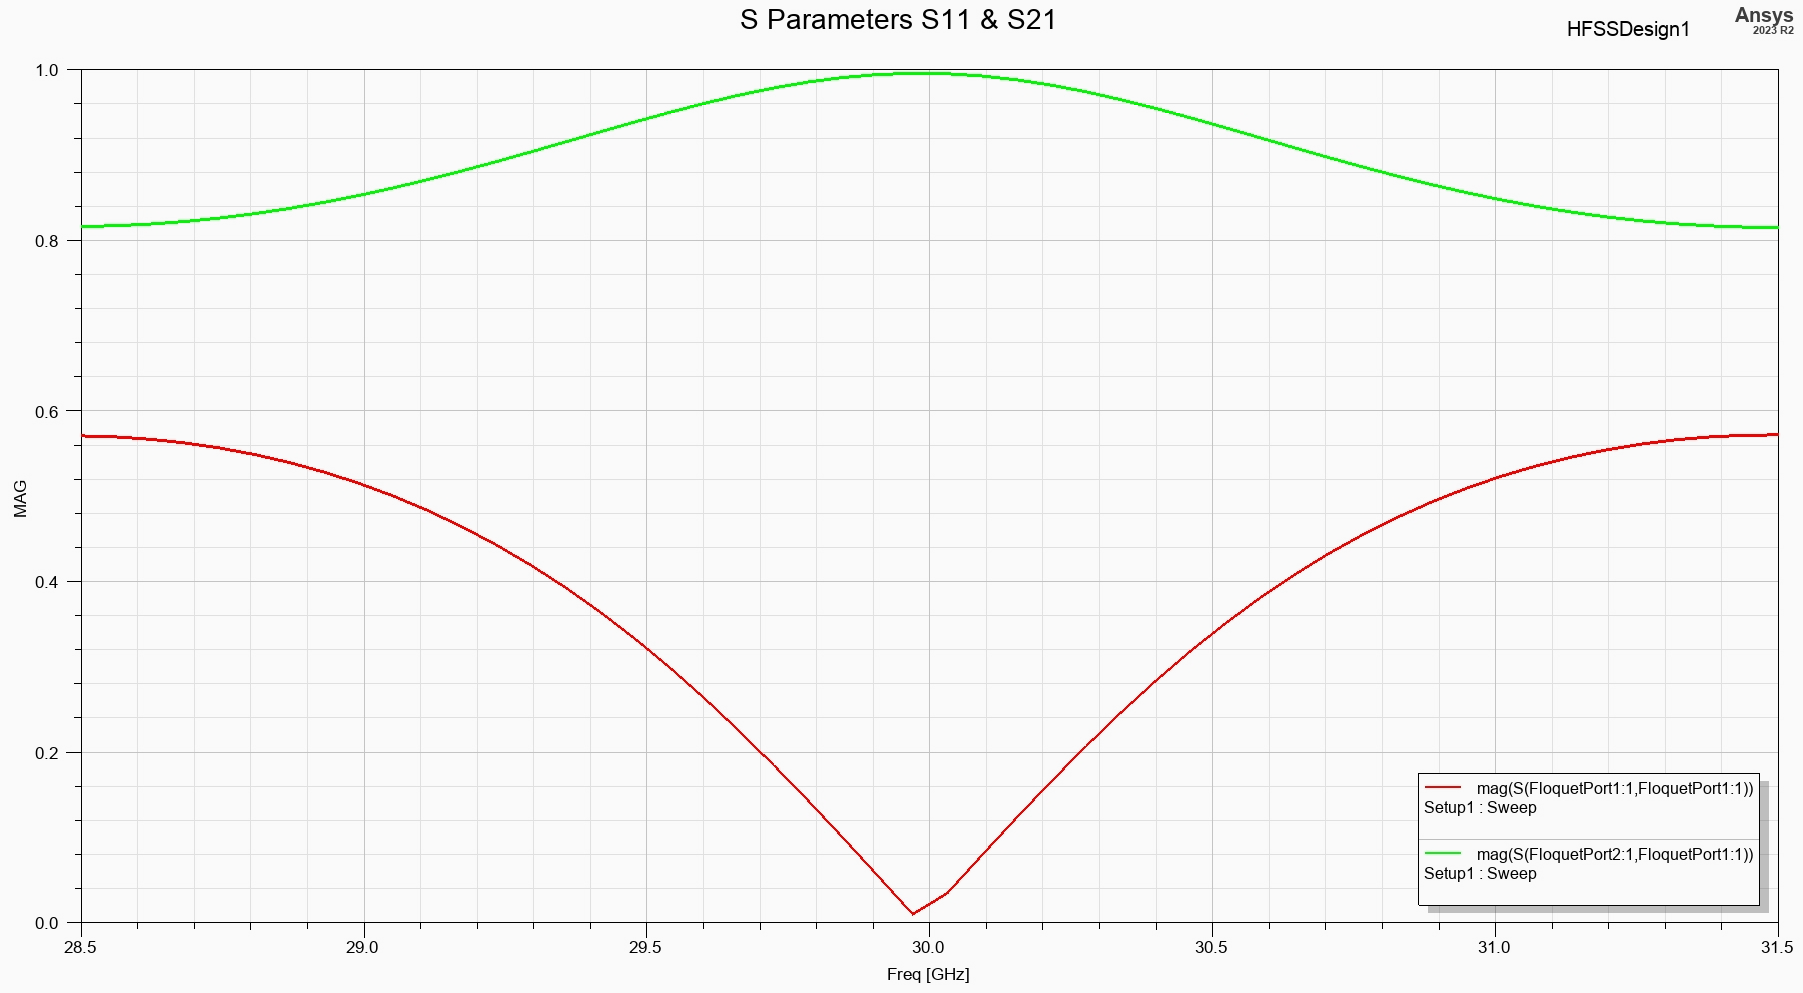
\includegraphics[width=17cm]{./images/Go1_5-9_final.png}
    \caption{S11 ans S21 results}
    \label{fig:S11_21}
  \end{figure}
\end{center}

This example in fig. \ref{fig:S11_21} shows the S-parameters of the design. The materials used are Silicon-Dioxide for the base, a customized teflon derivative with permitivitty 2, and embedded in vacuum.


%%%%%%%%%%%%%%%%%%%%%%%%%%%%%%%%%%%%%%%%%%%%%%%%%%%%%%%%%%%%%%%%%%%%%%%%%%%%%%%%%%%%%%%%%%%%%%%%%%%

\begin{figure}[ht]
\centering
% First row, left image
\begin{subfigure}[b]{0.45\textwidth}
  \centering
  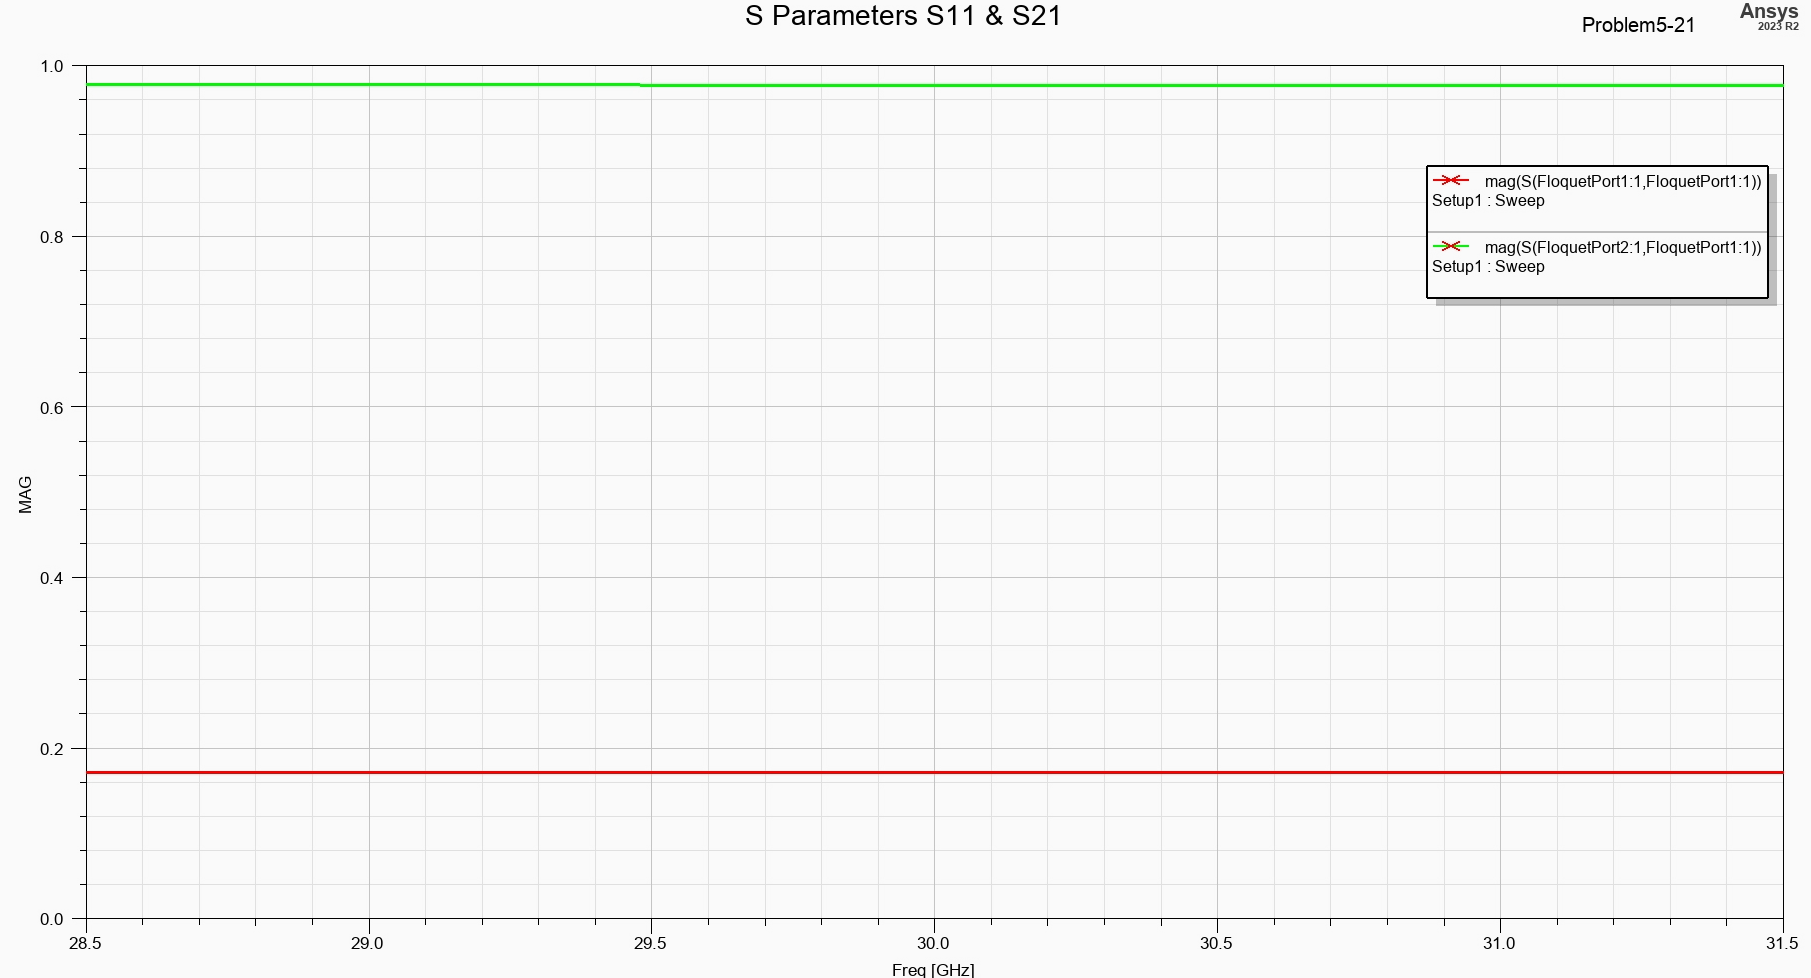
\includegraphics[width=\textwidth]{./images/S11_21_teflon_alone.png}
  \caption{Teflon alone}
  \label{fig:teflon}
\end{subfigure}
\hfill % This adds some space between the two subfigures
% First row, right image
\begin{subfigure}[b]{0.45\textwidth}
  \centering
  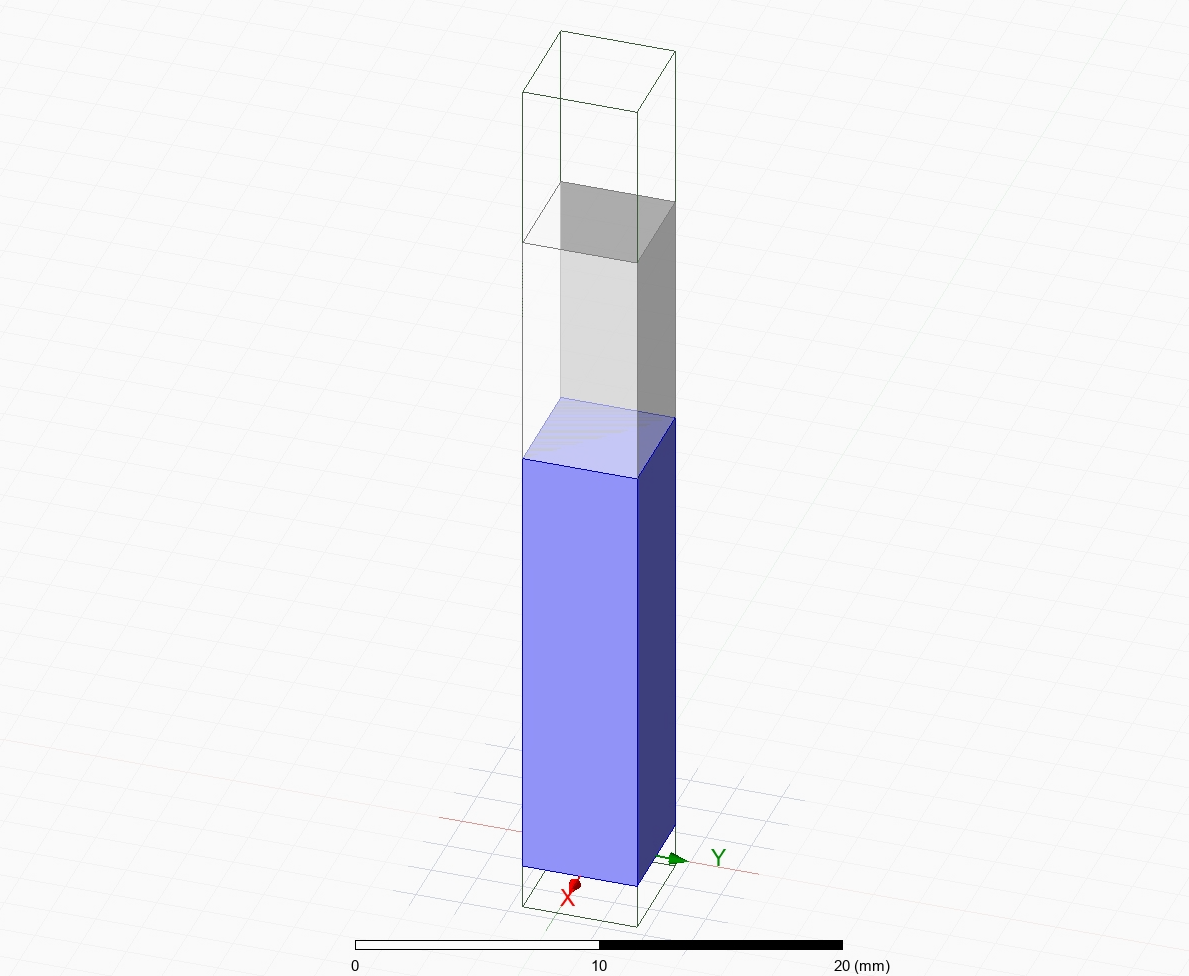
\includegraphics[width=\textwidth]{./images/Go1_5-9_model.png}
  \caption{3D model in Ansys}
  \label{fig:model}
\end{subfigure}

% Second row, left image
\begin{subfigure}[b]{0.45\textwidth}
  \centering
  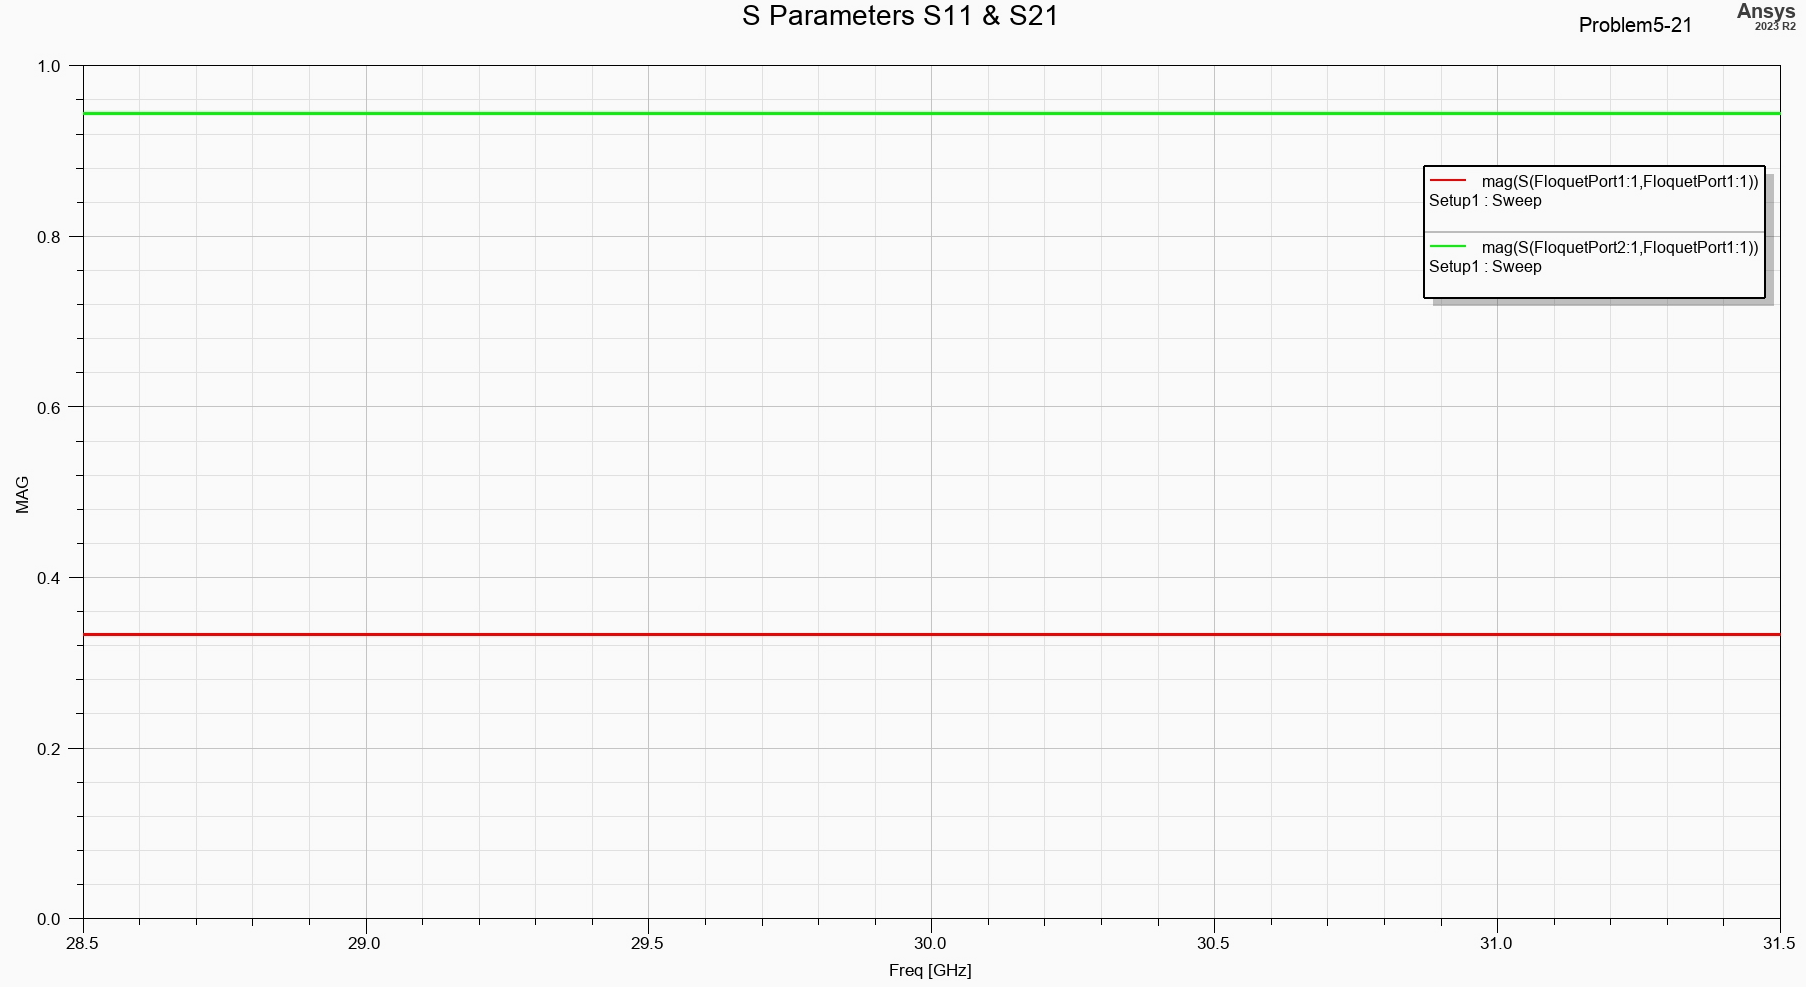
\includegraphics[width=\textwidth]{./images/S11_21_Si-O2_alone.png} 
  \caption{Si-O2 alone}
  \label{fig:sio2}
\end{subfigure}
\hfill % This adds some space between the two subfigures
% Second row, right image
\begin{subfigure}[b]{0.45\textwidth}
  \centering
  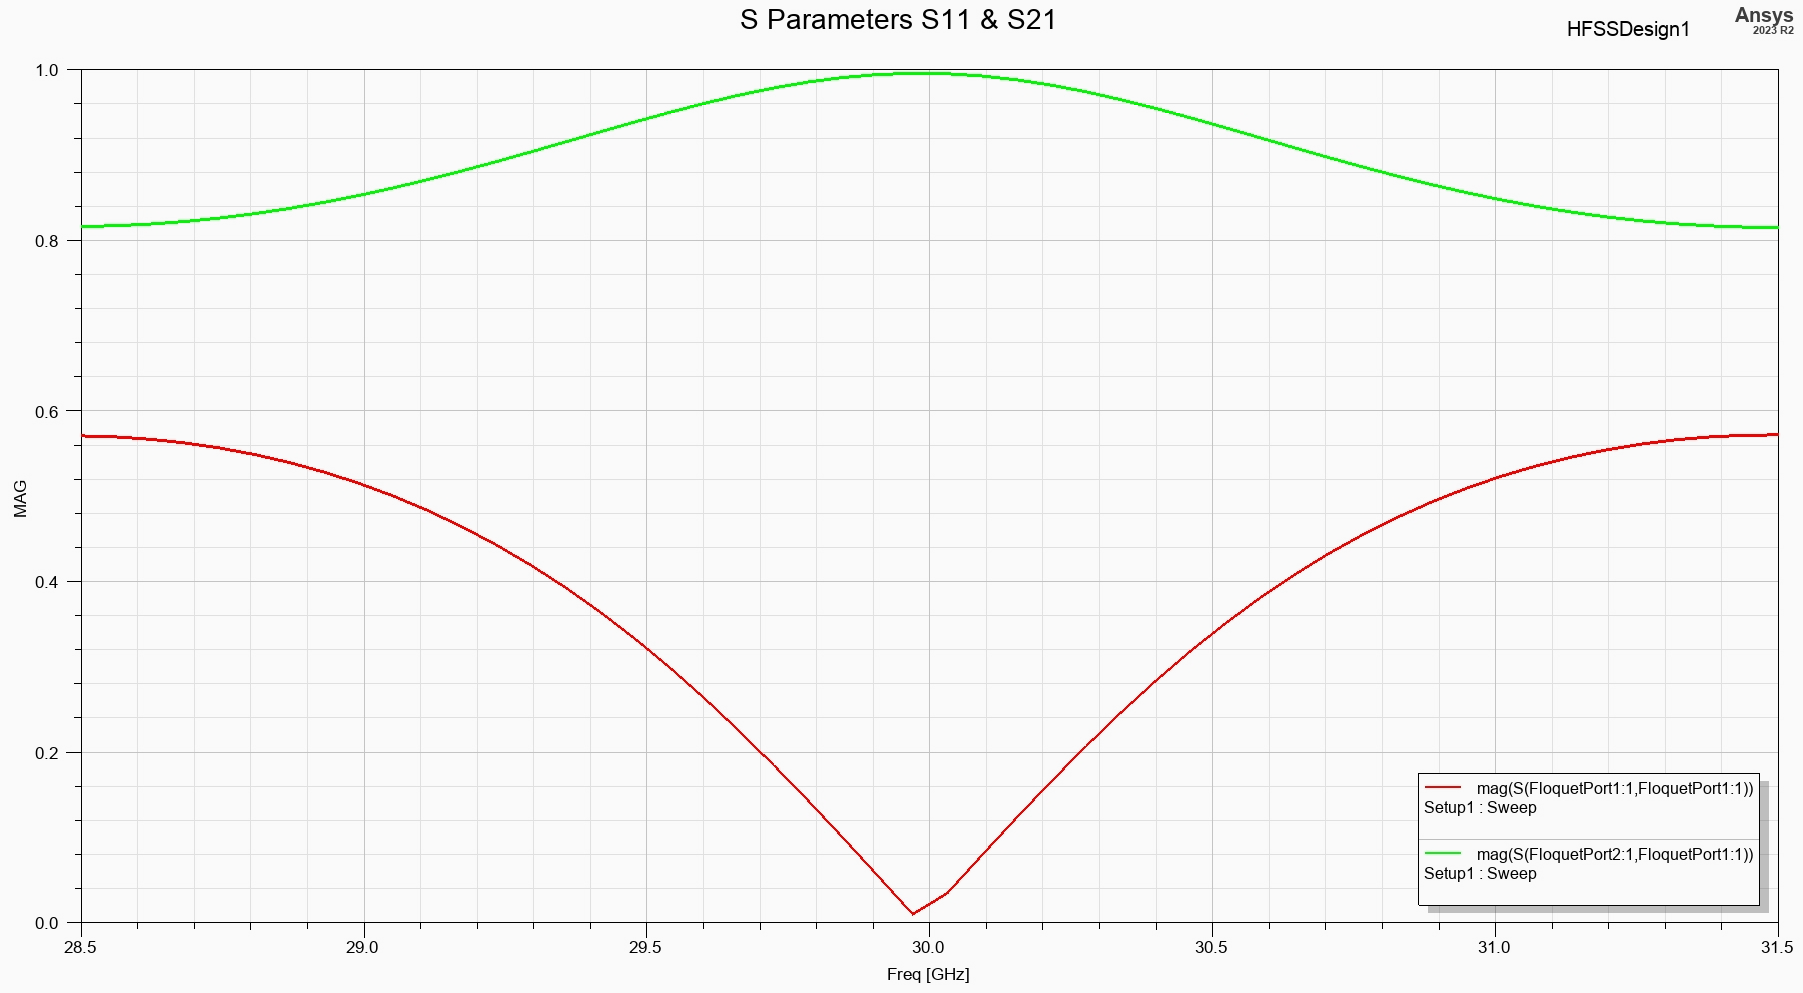
\includegraphics[width=\textwidth]{./images/Go1_5-9_final.png}
  \caption{Combined together}
  \label{fig:both_materials}
\end{subfigure}

\caption{Collection of design results}
\label{fig:collection}
\end{figure}


%%%%%%%%%%%%%%%%%%%%%%%%%%%%%%%%%%%%%%%%%%%%%%%%%%%%%%%%%%%%%%%%%%%%%%%%%%%%%%%%%%%%%%%%%%%%%%%%%%%
\newpage
Above in this figure, we can see the results agree with what we expected. Using a permitivitty of 2 cancels out the reflections. The design used $\approx 10mm$ for the thickness of the teflon.
\begin{align*}
  \lambda &= \frac{v_p}{f\sqrt{\mu\epsilon}}\\
  \lambda &= \frac{c}{f} = \frac{3e^8}{3e^{10}}\\
  \lambda &= 10 [mm]
\end{align*}
\newpage
\section*{Problem 5.21}
A uniform plane wave traveling in a lossless dielectric is incident normally on a flat interface formed by the presence of air. For $\epsilon_r$ ’s of 2.56, 4, 9, 16, 25, and 81:
\begin{itemize}
\item[(a)] Determine the critical angles.\\
  \begin{align*}
    \theta_i \geq \theta_c &= \sin{^{-1}\left(\sqrt{\frac{\mu_2\epsilon_2}{\mu_1\epsilon_1}}\right)}
  \end{align*}
\item[(b)] Find the Brewster angles if the wave is of parallel polarization.
  \begin{align*}
    \theta_B &= \tan{^{-1}\left(\sqrt{\frac{\epsilon_2}{\epsilon_1}}\right)}\\
    \theta_B &= \cos{^{-1}\left(\sqrt{\frac{\epsilon_1}{\epsilon_1 + \epsilon_2}}\right)}\\
    \theta_B &= \sin{^{-1}\left(\sqrt{\frac{\epsilon_2}{\epsilon_1 + \epsilon_2}}\right)}
  \end{align*}
\item[(c)] Compare the critical and Brewster angles found in parts (a) and (b).
\item[(d)] Plot the magnitudes of the reflection coefficients for both perpendicular, $|\Gamma_{\perp}|$ , and parallel, $|\Gamma_{\parallel}|$, polarizations versus incidence angle.
\item[(e)] Plot the phase (in degrees) of the reflection coefficients for both perpendicular
and parallel polarizations versus incidence angle.
\end{itemize}

% References (if any)
\bibliographystyle{plain}
\bibliography{references/references} 

\end{document}

%%% Local Variables:
%%% mode: LaTeX
%%% TeX-master: t
%%% End:
